\documentclass[a4j]{jarticle}
\usepackage{ascmac}
\usepackage{comment}
\usepackage{url}
\usepackage{amsmath, amssymb, amsfonts, latexsym }
\usepackage[dvipdfmx]{graphicx}
\usepackage{listings,jvlisting, jlisting}
\usepackage[hang,small,bf]{caption}
\usepackage[subrefformat=parens]{subcaption}
\captionsetup{compatibility=false}

\lstset{
  basicstyle={\ttfamily},
  identifierstyle={\small},
  commentstyle={\smallitshape},
  keywordstyle={\small\bfseries},
  ndkeywordstyle={\small},
  stringstyle={\small\ttfamily},
  frame={tb},
  breaklines=true,
  columns=[l]{fullflexible},
  numbers=left,
  xrightmargin=0zw,
  xleftmargin=3zw,
  numberstyle={\scriptsize},
  stepnumber=1,
  numbersep=1zw,
  lineskip=-0.5ex
}

\begin{document}

\vfill
\begin{screen}
  \begin{center}
    \huge\bf 実験　レポート2\\
    \vspace{5mm}
    \large\bf
    学籍番号　2022311042 \ 名前 神野友哉\\
    \today
  \end{center}
\end{screen}
\thispagestyle{empty}
%%目次
\tableofcontents

\newpage
% "%"同士に挟まれた行に書けばいいよ
\subsection{講義時間以外の取り組み時間}
%
実験自体は\ 9\ ～\ 10\ 時間、レポート作成込みで\ 30\ 時間程度
%
\subsection{自己評価}
%
S
%


\newpage
\section{課題\ 1}
1.3.1節で作成したロボットに新たに可動部品を追加し、レンダリングしなさい。ただし、まだ紹介されていない3ds\ Max\ の機能を\ 2\ つ以上利用すること
\subsection{結果}
%
以下の図\ref{fig:d} を製作することが出来た。新しく追加した可動部品としては、図\ref{fig:kct}の頭部上の王冠と、図\ref{fig:kkt}の両肩に翼を模した板である。また、左翼は右翼の複製であり、パラメータは共通していて図\ref{fig:kRt}となっている。
%

% 下のコードで画像を二枚組にする。newpage は任意
\begin{figure}[htbp]
  \begin{minipage}{0.5\textwidth}
    \begin{center}
      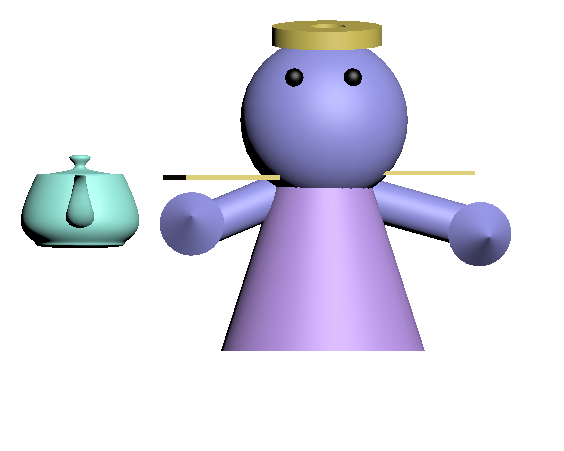
\includegraphics[width=70mm, height=50mm]{no/mydoll.png}
    \end{center}
    \caption{作成したロボット}
    \label{fig:d}
  \end{minipage}
  \begin{minipage}{0.5\textwidth}
    \begin{center}
      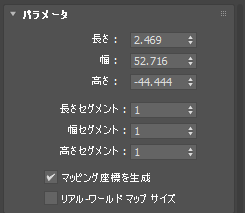
\includegraphics[width=70mm, height=50mm]{no/kataR-t.png}
    \end{center}
    \caption{翼のパラメータ}
    \label{fig:kRt}
  \end{minipage}
\end{figure}

図\ref{fig:kkLt}, \ref{fig:kkRt}の基点は首の周りに調整されている。

\begin{figure}[htbp]
  \begin{minipage}{0.5\textwidth}
    \begin{center}
      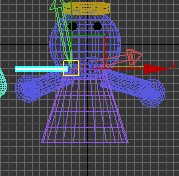
\includegraphics[width=70mm, height=50mm]{no/kitenkataL-t.png}
    \end{center}
    \subcaption{左翼}
    \label{fig:kkLt}
  \end{minipage}
  \begin{minipage}{0.5\textwidth}
    \begin{center}
      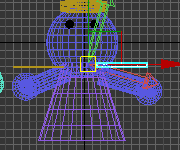
\includegraphics[width=70mm, height=50mm]{no/kitenkataR-t.png}
    \end{center}
    \subcaption{右翼}
    \label{fig:kkRt}
  \end{minipage}
  \caption{翼の基点}
  \label{fig:kkt}
\end{figure}

\newpage
図\ref{fig:ct}は王冠のパラメータである。

\begin{figure}[htbp]
  \begin{minipage}{0.5\textwidth}
    \begin{center}
      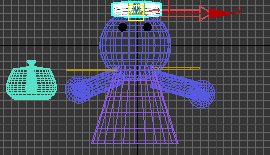
\includegraphics[width=70mm, height=50mm]{no/kitencrown-t.png}
    \end{center}
    \caption{王冠の基点}
    \label{fig:kct}
  \end{minipage}
  \begin{minipage}{0.5\textwidth}
    \begin{center}
      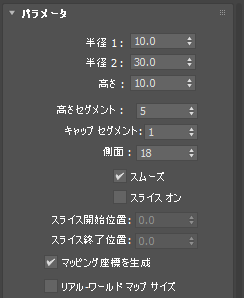
\includegraphics[width=70mm, height=50mm]{no/crown-t.png}
    \end{center}
    \caption{王冠のパラメータ}
    \label{fig:ct}
  \end{minipage}
\end{figure}

\newpage
\section{課題\ 2}
課題\ 1 \ で利用した\ 3ds\ Max\ の機能について、その特徴、役割、操作方法などを解説しなさい。
\subsection{解説}
%
翼では\verb|[ボックス]|を、王冠では\verb|[チューブ]|を用いた。
前者は、縦、横、高さ等を指定して直方体を作成できる。その立体自体の汎用性によって、\ 3\ DCG作成に使われる頻度は比較的高いと考えられる。各頂点周辺を切り取りや、引き延ばし、面によって色を塗る等の操作も可能である。
後者は、外円半径、内円半径、高さ等を指定して、ストローや導管等に用いられる円筒を作成できる。\verb|[円柱]|との差別点は、空洞となる内円部分の半径をパラメータで指定することで、操作し易い点である。
%

\newpage
\section{課題\ 3}
この実験では人間が手作業で行う\ CG\ 制作を体験しているが、最近では生成系\ AI\ を利用して\ CG\ を製作することも盛んに行われている。人間が手作業で行う\ CG\ 製作と生成系\ AI\ が作成する
\ CG\ を比較して、人間でなければ作成できない部分、人間では作成できない部分について述べなさい。
\subsection{考察}
%
ウェブサイトAismiley(2023)によると、AIの強みは膨大なデータを素早く処理でき、類似の作業を高速かつ一貫して実行できるという\cite{Aismiley}。
これにより、多くのコンテンツを短時間で生成できると考えられる。この点、人間では作成できない様な巨大\ CG\ 作成等や、短期間での量に重きを置いた製作
に活用されるのではないか。 また、同ウェブサイトには、AIの短所も指摘されていて、AIは「過去のデータをもとに作業を行うこと」を得意としている、
つまり、人間が開拓してきたアイデアに基づかざるを得ないという\cite{Aismiley}。逆に言えば、
今までにない独創的なアイデアを新規開拓することは、人間でなければ作成できない部分だろう。
%

\newpage
\section{課題\ 4}
次の合成オブジェクトタイプからひとつを選んでそれを生かした\ CG\ を作成し、その画像を使って特徴、役割を解説しなさい。
\begin{itemize}
  \item[■] モーフ
  \item[■] スキャッタ
  \item[■] コンフォーム
  \item[■] 接続
  \item[■] シェイプマージ
  \item[■] ロフト
  \item[■] ブロッブメッシュ
\end{itemize}
\subsection{結果}
%
図\ref{fig:scatta}のように、\verb|[スキャッタ]|を活用することで、\verb|[円柱]|を\verb|[チューブ]|の外・内円周上に等間隔になるように立てた。
\begin{figure}[htbp]
  \begin{minipage}{0.3\textwidth}
    \begin{center}
      \includegraphics[width=40mm]{yusou/2-4-kadai4-spire.png}
    \end{center}
    \subcaption{作成した CG}
    \label{fig:CGmade}
  \end{minipage}
  \begin{minipage}{0.3\textwidth}
    \begin{center}
      \includegraphics[width=40mm]{yusou/2-4-kadai4-bunpai.png}
    \end{center}
    \subcaption{すべての頂点に配置をチェック}
    \label{fig:CGbunpai}
  \end{minipage}
  \begin{minipage}{0.3\textwidth}
    \begin{center}
      \includegraphics[width=40mm]{yusou/2-4-kadai4-cylinder.png}
    \end{center}
    \subcaption{元となったチューブと分配対象の柱}
    \label{fig:CGcylinder}
  \end{minipage}
  \caption{スキャッタを用いた図}
  \label{fig:scatta}
\end{figure}
%
\subsection{特徴}
%
図\ref{fig:CGcylinder}のように、用意した二つのオブジェクトのうち、一方を分配オブジェクト、もう一方を配置元\verb|(便宜上)|とする。配置元に分配オブジェクトを大量に分散配置することが可能である。また、特定の面上や図\ref{fig:CGbunpai}のように頂点上のみに分配させることも可能であり、今回は全ての頂点に配置させている。
%
\subsection{役割}
%
\verb|[スキャッタ]|を用いずに一つ一つ地道に配置する方法で同じ\ CG\ を作成するよりも、当然ながら労力的時間的に効率がよい。そのため、この\verb|[スキャッタ]|を用いるべき身近な例では、植物のイバラや森の木々等、大量に無造作に配置しても問題がないと見做される場合や、図\ref{fig:CGmade}のように一定の規則で配置させ人工物らしく作りたい場合である。
%

\newpage
\section{課題\ 5}
%
バンプに似た機能にディスプレイスメントマップがある。それぞれどのような違いがあるのか、どういったモデル・どういった表現に向いているのかなどその特徴を述べよ。
%
\subsection{違い}
%
\ CGWORLD.jp\ (2016)によると、ディスプレイスメントマップは実際にモデルを変更するという\cite{cgworld}。具体的には、モデルにジオメトリを追加することにより、テクスチャの物理的な凹凸の表現を可能にする。半面、計算コストが高くなる傾向がある。一方、バンプマップはジオメトリを追加せずに凹凸があるかのように見せるという\cite{cgworld}。具体的には、グレースケールで凹凸を再現するディテールを追加する。このバンプマップは、ディスプレイスメントマップと比較して計算コストが低い傾向がある。
%
\subsection{向いているモデル・表現}
%
\subsubsection{ディスプレイスメントマップ}
%
地形の詳細な凹凸や高度変化の表現が重要な場合。例えば、土地や山地の表現、キャラクターモデリングにおけるシワなどの細かい表現をリアルに再現する際に適していると考えられる。
%
\subsubsection{バンプマップ}
%
低負荷でモデルを作りたい場合やディスプレイスメントマップのようにモデルを変更する処理が忌避される場合。 また、壁や床などの表面に細かな模様や凹凸を追加して、リアルな質感を表現したい場合に適していると考えられる。具体的には、リアルタイムレンダリングでゲームエンジン等に使われている。
%
\subsubsection{バンプマップでのレンダリング}
%
図\ref{fig:bmpmap}は実際にオブジェクトにバンプを適用した図である。適当なボックスを作成し、図\ref{fig:bricks}のテクスチャを適用、\verb|[特殊なマップ]|から\verb|[バンプマップ]|の数字を\ 0.3\ 、\ 1.0\ 、\ 10.0\ に設定し、各々レンダリングを行った。`
\begin{figure}[htbp]
   \begin{center}
     \includegraphics[width=70mm]{bump.png}
  `\end{center}
   \caption{レンガのテクスチャ}
   \label{fig:bricks}
\end{figure}
\begin{figure}[htbp]
  \begin{minipage}{0.33\textwidth}
    \begin{center}
      \includegraphics[width=70mm]{bump-003.png}
    \end{center}
    \subcaption{bump : 0.3}
    \label{fig:bmp003}
  \end{minipage}
  \begin{minipage}{0.33\textwidth}
    \begin{center}
      \includegraphics[width=70mm]{bump-010.png}
    \end{center}
    \subcaption{bump : 1.0}
    \label{fig:bmp010}
  \end{minipage}
  \begin{minipage}{0.33\textwidth}
    \begin{center}
      \includegraphics[width=70mm]{bump-100.png}
    \end{center}
    \subcaption{bump : 10.0}
    \label{fig:bmp100}
  \end{minipage}
  \caption{バンプマップを用いた図}
  \label{fig:bmpmap}
\end{figure}
%

\newpage
\section{実験\ 1-1}
スプラインを作成するときにクリックしていく頂点を時計回り/反時計回りに選択してモデリングした時、概観、ポリゴン数、レンダリング時間などに
どういった差異が出るかを確認しなさい。ただし、レンダリング設定で\verb$[範囲]$ を\ 0 \
、\verb$[終端]$ を\ 99\ にしてレンダリングし、その\ 1 \ 枚当たりの平均時間を求めること。
\subsection{目的}
%
スプラインの作成の際の頂点の選び方による、モデリングへの影響を調査する
%
\subsection{方法や条件}
%
\subsubsection{正方形(クリックのみ)}
\begin{description}
\item{手順１} \verb|[作成]|パネルの\verb|[シェイプ]|を表示
\item{手順２} \verb|[スプライン]|の\verb|[オブジェクトタイプ]|で\verb|[ライン]|を選択
\item{手順３} \verb|[補間]|の\verb|[ステップ数:]|を６にし、\verb|[最適化とアダプティブ]|のチェックを外し、\verb|[作成方法]|の\verb|[初期タイプ]|を\verb|[コーナー]|に、\verb|[ドラッグタイプ]|を\verb|[ベジェ]|にする
\item{手順４} ビューポート内で、方眼の格子点を座標に見立て、適当に原点を仮定し、その相対座標で、\verb|{-4, 0}|, \verb|{0, 4}|, \verb|{4, 0}|, \verb|{0, -4}|の順に頂点位置を設置(左クリック)する
\item{手順５} 最後の頂点位置を再び置くと、スプラインを閉じるか問うウィンドウが出るので、許可して終了する
\item{手順６} 作成したスプラインを選択し、修正パネルの\verb|[モディファイヤリスト]|から\verb|[レイズ]|を選択
\item{手順７} \verb|[回転角度:]|を\ 360\ \verb|[セグメント]|を\ 16\ に設定
\item{手順８} \verb|[方向]|に\verb|[Y]|を、\verb|[位置合わせ]|に\verb|[最大]|を設定
\item{手順９} メインメニューの\verb|[レンダリング]|の\verb|[レンダリング設定]|を選択
\item{手順１０} 開いたダイアログの\verb|[範囲]|を\ 0\ 、\verb|[終点]|を\ 99\ にする
\item{手順１１} \verb|[レンダリング設定]|の右上にある\verb|[レンダリング]|ボタンをクリック
\item{手順１２} メインメニューの\verb|[ファイル]|から\verb|[シーン情報(U)]|を選択し、ポリゴン数、レンダリング時間を確認する
\item{手順１３} 手順\ 4\ の頂点の取り方を逆順にして、再度、手順\ 1 ～\ 12\ を行う
\item{手順１４} レンダリング画像から概観を比較
\end{description}
\subsubsection{三角形(ドラッグのみ)}
\begin{description}
\item{手順１} 正方形\verb|(クリックのみ)|の手順\ 1\ ～\ 3\ を行う
\item{手順２} ビューポート内で、方眼の格子点を座標に見立て、適当に原点を仮定し、その相対座標で、\verb|{-1, 0}|から\verb|{1, 1}|まで、\verb|{1, 1}|から\verb|{1, -1}|まで、\verb|{1, -1}|から\verb|{-1, 0}|までの三つにおいてドラッグして離すを行う
\item{手順３} 正方形\verb|(クリックのみ)|の手順\ 5\ から\ 12\ を実行する
\item{手順４} 手順\ 2\ を逆順にして、手順\ 1\ ～\ 3\ を行う
\item{手順５} レンダリング画像から概観を比較
\end{description}
%
\subsection{結果}
%
スプライン時計回り/反時計回りでのモデリングの概観は、正方形\verb|(クリックのみ)|を実施した図\ref{fig:cw}, \ref{fig:ccw}を観察したところ、差異が見られなかった。また、ポリゴン数はそれぞれ、\ 13660\ ,\ 13200\ であった。\ 1\ 枚辺りのレンダリング平均時間は、それぞれ、\ 0.49s\ ,\ 0.53s\ だった。
\begin{figure}[htbp]
  \begin{minipage}{0.5\textwidth}
    \begin{center}
      \includegraphics[width=70mm]{tyoutennsikaku.png}
    \end{center}
    \caption{(正方形クリックのみ)頂点位置 : 時計}
    \label{fig:cw}
  \end{minipage}
  \begin{minipage}{0.5\textwidth}
    \begin{center}
      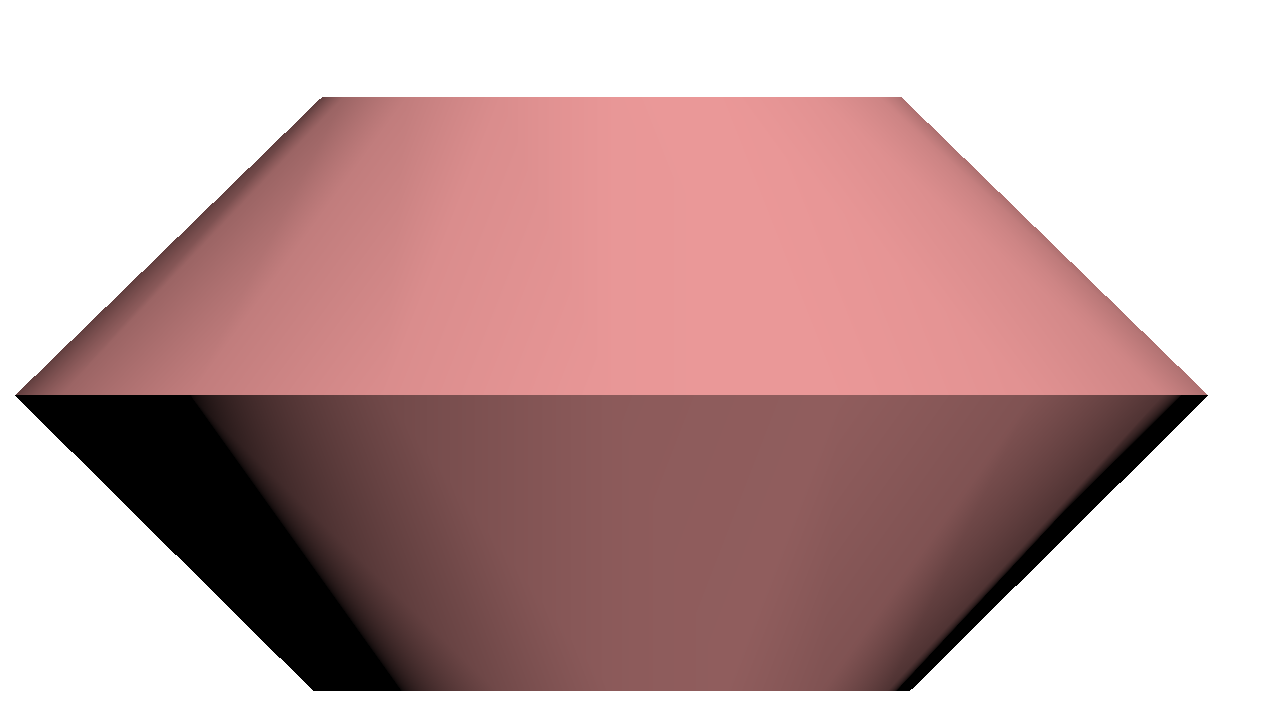
\includegraphics[width=70mm]{no/clockwise-raise.png}
    \end{center}
    \caption{(正方形クリックのみ)概形 ; 時計}
    \label{fig:cwa}
  \end{minipage}
\end{figure}
\begin{figure}[htbp]
  \begin{minipage}{0.5\textwidth}
    \begin{center}
      \includegraphics[width=70mm]{tyoutennsikaku.png}
    \end{center}
    \caption{(正方形クリックのみ)頂点位置 : 反時計}
    \label{fig:ccw}
  \end{minipage}
  \begin{minipage}{0.5\textwidth}
    \begin{center}
      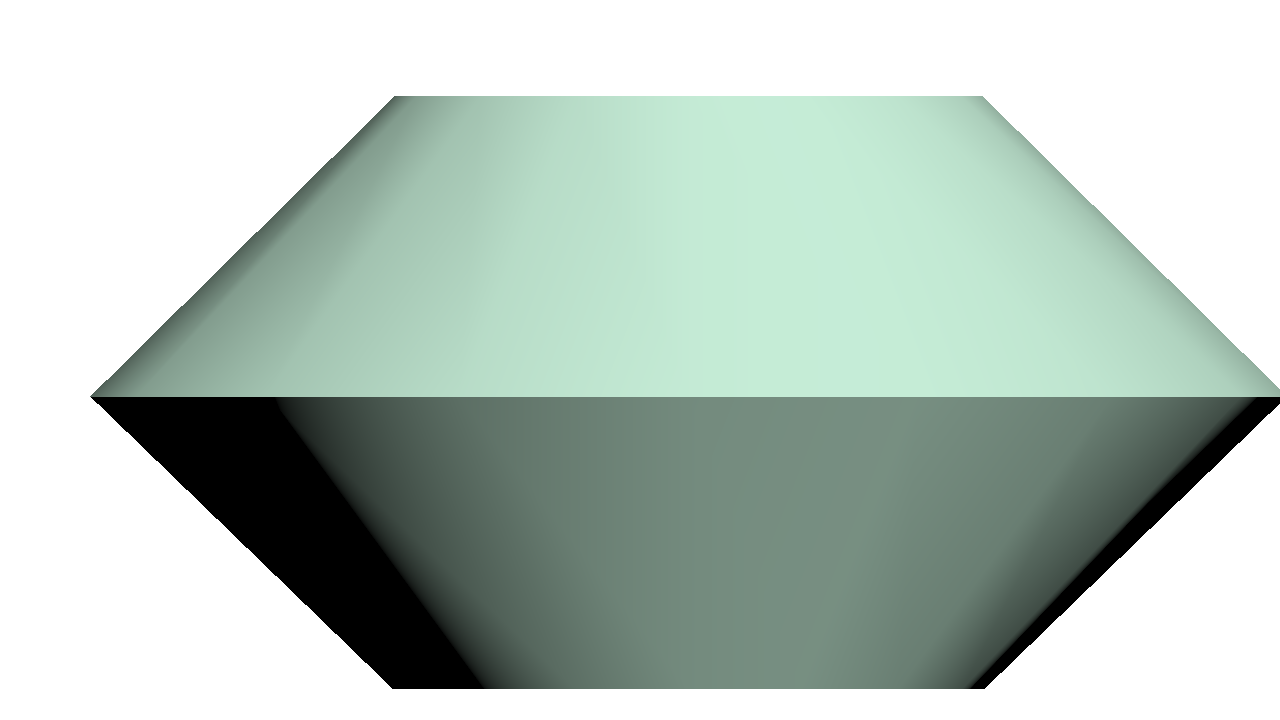
\includegraphics[width=70mm]{no/counterclockwise-raise.png}
    \end{center}
    \caption{(正方形クリックのみ)概形 : 反時計}
    \label{fig:ccwa}
  \end{minipage}
\end{figure}

三角形\verb|(ドラッグのみ)|を実施した図\ref{fig:tcw}, \ref{fig:tccw}を観察したところ、スプライン曲線の向きが異なっていることが解かる。さらに、図\ref{fig:tcwa}, \ref{fig:tccwa}は概観であるが、両方ともドーナツ状であるが、穴の開き具合が大きく異なっていることが解る。両方ともポリゴン数とレンダリング時間は、\ 672\ 、 0.08s であった。

\begin{figure}[htbp]
  \begin{minipage}{0.5\textwidth}
    \begin{center}
      \includegraphics[width=70mm]{tyoutentokei.png}
    \end{center}
    \caption{(三角形ドラッグのみ)頂点位置 : 時計}
    \label{fig:tcw}
  \end{minipage}
  \begin{minipage}{0.5\textwidth}
    \begin{center}
      \includegraphics[width=70mm]{notsquare-clock-008.png}
    \end{center}
    \caption{(三角形ドラッグのみ)概形 ; 時計}
    \label{fig:tcwa}
  \end{minipage}
\end{figure}
\begin{figure}[htbp]
  \begin{minipage}{0.5\textwidth}
    \begin{center}
      \includegraphics[width=70mm]{tyoutenhanntokei.png}
    \end{center}
    \caption{(三角形ドラッグのみ)頂点位置 : 反時計}
    \label{fig:tccw}
  \end{minipage}
  \begin{minipage}{0.5\textwidth}
    \begin{center}
      \includegraphics[width=70mm]{notsquare-counterclock-008.png}
    \end{center}
    \caption{(三角形ドラッグのみ)概形 : 反時計}
    \label{fig:tccwa}
  \end{minipage}
\end{figure}
%
\subsection{考察}
%
正方形\verb|(クリックのみ)|の概観に差異が見られなかった理由として、ドラッグを使わないで作成したため、曲線を含まなかったことが原因と考えられる。なぜなら、守屋悦朗(2023)によるとスプライン曲線は、元の曲線を小区間に分けて、各々で曲線を近似しているという\cite{moriya}\verb|(|ここから\verb|[補間]|の数字が頂点間の部分曲線を区分する個数であると仮定する\verb|)|。正方形の辺のように直線を引いた場合、スプライン曲線上どの小区間の傾きも、直線と同じ傾きで一定になるのではないか。また、図\ref{fig:tcw}, \ref{fig:tccw}を観察すると、時計回りに配置した場合は進行方向左に逸れ、反時計回りの場合は右に逸れていると考えられるため、作成したい\ CG\ でスプライン曲線を用いるとき、その点に注意する必要があるのではないか。
%


\newpage
\section{実験\ 1-2}
スプラインのステップ数を\ 2\ ～\ 20\ に\ 2\ ずつ変更してモデリングした時、概観、ポリゴン数、レンダリング時間などにどういった差異が出るかを確認しなさい。
\subsection{目的}
%
スプラインのステップ数を変化させた場合の、モデリングへの影響を調査する
%
\subsection{方法や条件}
%
実験\ 1-1\ 正方形を主に実験するが、比較として実験\ 1-1\ 三角形も軽く確かめる。
\subsubsection{正方形(クリックのみ)}
\begin{description}
\item[手順１] 実験\ 1-1\ 正方形\verb|(クリックのみ)|の手順\ 1\ ～\ 8\ を行う
\item[手順２] \verb|[モデファイヤリスト]|の下の欄からラインを選択しステップ数の数字を\ 2\ ～\ 20\ に\ 2\ ずつ変更する。各々の数字で、\verb|[モデファイヤリスト]|の下の欄からレイズを選択し直し、実験\ 1-1\ 正方形\verb|(クリックのみ)|の手順\ 9\ ～\ 12\ を実施する動作を行う
\item[手順３] レンダリング画像から概観を比較
\end{description}
\subsubsection{三角形(ドラッグのみ)}
\begin{description}
\item[手順１] 実験\ 1-1\ 三角形\verb|(ドラッグのみ)|の手順\ 1\ ～\ 3\ を行う
\item[手順２] \verb|[モデファイヤリスト]|の下の欄からラインを選択しステップ数の数字を\ 2\ 、\ 11\ 、\ 20\ に変更する。各々の数字で、\verb|[モデファイヤリスト]|の下の欄からレイズを選択し直し、実験\ 1-1\ 正方形\verb|(クリックのみ)|の手順\ 9\ ～\ 12\ を実施する動作を行う
\item[手順３] レンダリング画像から概観を比較 
\end{description}
%
\subsection{結果}
%
正方形の場合の図\ref{fig:seihou1no1}を綿密に比較しても概観に差異は見受けられなかった。また、表\ref{table:si} からポリゴン数は、ステップ数が\ 2\ 増加するに連れて\ 256\ 増加すると解かる。レンダリング時間については、ステップ数\ 2\ ～\ 20\ の比較で、外れ値のステップ数が\ 10\ の場合を除いて、\ 0.72\ ～\ 0.74\ 秒であった。
\begin{figure}[htbp]
  \begin{minipage}{0.5\textwidth}
    \begin{center}
      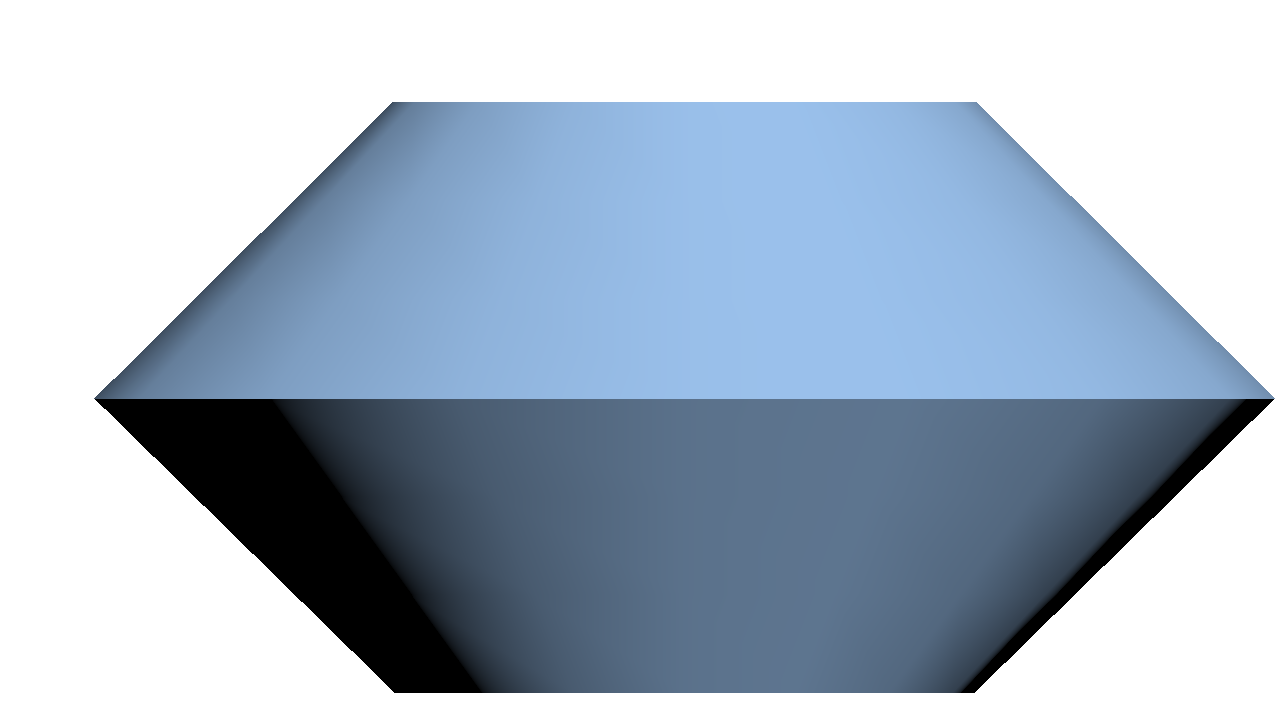
\includegraphics[width=70mm]{no/1-2-2-out.png}
    \end{center}
    \subcaption{ステップ数 : 2}
    \label{fig:st10}
  \end{minipage}
  \begin{minipage}{0.5\textwidth}
    \begin{center}
      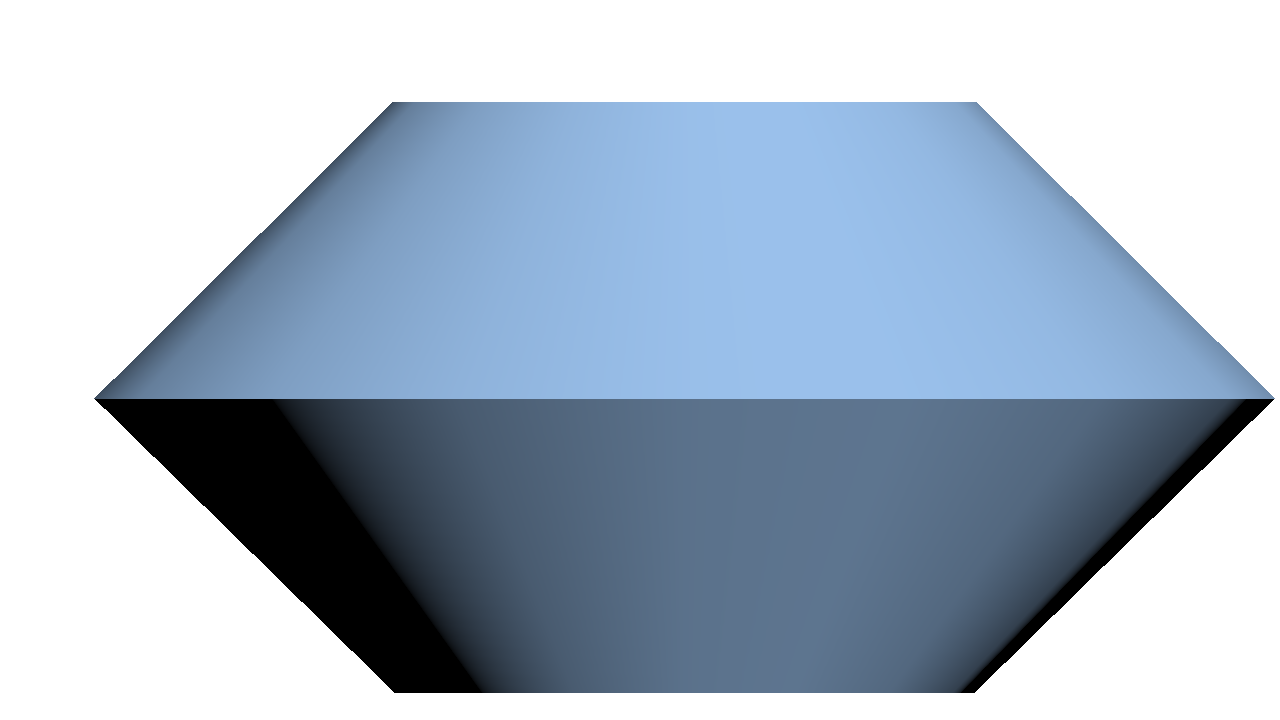
\includegraphics[width=70mm]{no/1-2-20-out.png}
    \end{center}
    \subcaption{ステップ数 : 20}
    \label{fig:st100}
  \end{minipage}
  \caption{正方形クリックのみ}
  \label{fig:seihou1no1}
\end{figure}

\begin{table}
  \caption{正方形の場合}
  \label{table:si}
  \centering
  \begin{tabular}{|c|c|c|}
  \hline
  ステップ数 & ポリゴン数 & レンダリング時間\verb|(s)| \\
  \hline
  2 & 13916 & 0.72 \\
  4 & 14172 & 0.72 \\
  6 & 14428 & 0.74 \\
  8 & 14684 & 0.73 \\
  10 & 14940 & 0.85 \\
  12 & 15196 & 0.73 \\
  14 & 15452 & 0.74 \\
  16 & 15708 & 0.74 \\
  18 & 15964 & 0.74 \\
  20 & 16220 & 0.74 \\
  \hline
  \end{tabular}
\end{table}
三角形の場合は、図\ref{fig:tri1no1}より、段々とスリムになっていくような概観の変化が見受けられた。また表\ref{table:sa}からステップ数が\ 9\ 増加するごとに、\ 764\ 増加すると解かる。レンダリング時間も最大で0.01sの差であった。
\begin{figure}[htbp]
  \begin{minipage}{0.33\textwidth}
    \begin{center}
      \includegraphics[width=40mm]{no/notsquare-clock-step2-288-008.png}
    \end{center}
    \subcaption{ステップ数 : 2}
    \label{fig:st2}
  \end{minipage}
  \begin{minipage}{0.33\textwidth}
    \begin{center}
      \includegraphics[width=40mm]{no/notsquare-clock-step11-1152-009.png}
    \end{center}
    \subcaption{ステップ数 : 11}
    \label{fig:st11}
  \end{minipage}
  \begin{minipage}{0.33\textwidth}
    \begin{center}
      \includegraphics[width=40mm]{no/notsquare-clock-step20-2016-009.png}
    \end{center}
    \subcaption{ステップ数 : 20}
    \label{fig:st20}
  \end{minipage}
  \caption{三角形ドラッグのみ}
  \label{fig:tri1no1}
\end{figure}
\begin{table}
  \caption{三角形の場合}
  \label{table:sa}
  \centering
  \begin{tabular}{|c|c|c|}
  \hline
  ステップ数 & ポリゴン数 & レンダリング時間\verb|(s)| \\
  \hline
  2 & 288 & 0.08 \\
  11 & 1152 & 0.09 \\
  20 & 2016 & 0.09 \\
  \hline
  \end{tabular}
\end{table}
%
\subsection{考察}
%
ウェブサイト\ iPentec\ (2022)によると、スプラインのステップ数の値はスプライン曲線の滑らかに影響するという\cite{toritchi}。そのため、三角形の場合の図\ref{fig:11}が膨らんで見えたのが、粗い近似によるスプライン曲線を回転させ、立体の表面が平面的になったことが原因ではないかと考えられる。
また、正方形の場合の概観に差異が見られなかった原因も考察する。
頂点位置を正方形になるよう描いたことで、ステップ数の値の高低問わず辺が直線的で、角が直角になったため、概観に差異が見られなかったと考えられる。結果から、ポリゴン数の値をステップ数との数式で表せると考え、ポリゴン数を\ P\ 、ステップ数を\ S\ とすると、正方形の場合は
\begin{equation}
  P = 128S + 13660
\end{equation}
三角形の場合は、あくまで比較のため軽く検証したのみであるが、
\begin{equation}
  P = 96(S + 1)
\end{equation}
と考察される。
%

\newpage
\section{実験\ 1-3}
レイズのセグメント数を\ 10\ ～\ 100\ に\ 10\ ずつ変更してモデリングした時、概観、ポリゴン数、
レンダリング時間などにどういった差異が出るかを確認しなさい。
\subsection{目的}
%
レイズのセグメント数を変化させた場合の、モデリングへの影響を調査する
%
\subsection{方法や条件}
%
実験\ 1-1\ 正方形を主に実験するが、比較として実験\ 1-1\ 三角形も軽く確かめる
\subsubsection{正方形(クリックのみ)}
\begin{description}
\item[手順１] 実験\ 1-1\ 正方形\verb|(クリックのみ)|の手順\ 1\ ～\ 8\ を行う
\item[手順２] セグメント数の数字を\ 10\ ～\ 100\ に\ 10\ ずつ変更する。各々の数字で、各々の数字で実験\ 1-1\ 正方形\verb|(クリックのみ)|の手順\ 9\ ～\ 12\ を実施する動作を行う
\item[手順３] レンダリング画像から概観を比較 
\end{description}
\subsubsection{三角形(ドラッグのみ)}
\begin{description}
\item[手順１] 実験\ 1-1\ 三角形\verb|(ドラッグのみ)|の手順\ 1\ ～\ 3\ を行う
\item[手順２] セグメント数の数字を\ 10\ 、\ 55\ 、\ 100\ に変更する。各々の数字で、実験\ 1-1\ 正方形\verb|(クリックのみ)|の手順\ 9\ ～\ 12\ を実施する動作を行う
\item[手順３] レンダリング画像から概観を比較 
\end{description}
%
\subsection{結果}
%
正方形の場合は概観の差分は図\ref{fig:seihou1no2}を見ると、角が取れるような外観の変化だと解る。また、ポリゴン数は、表\ref{table:2}から、セグメント数が\ 10\ 増加するに連れて、ポリゴン数も\ 1120\ 増加している。
\begin{figure}[htbp]
  \begin{minipage}{0.5\textwidth}
    \begin{center}
      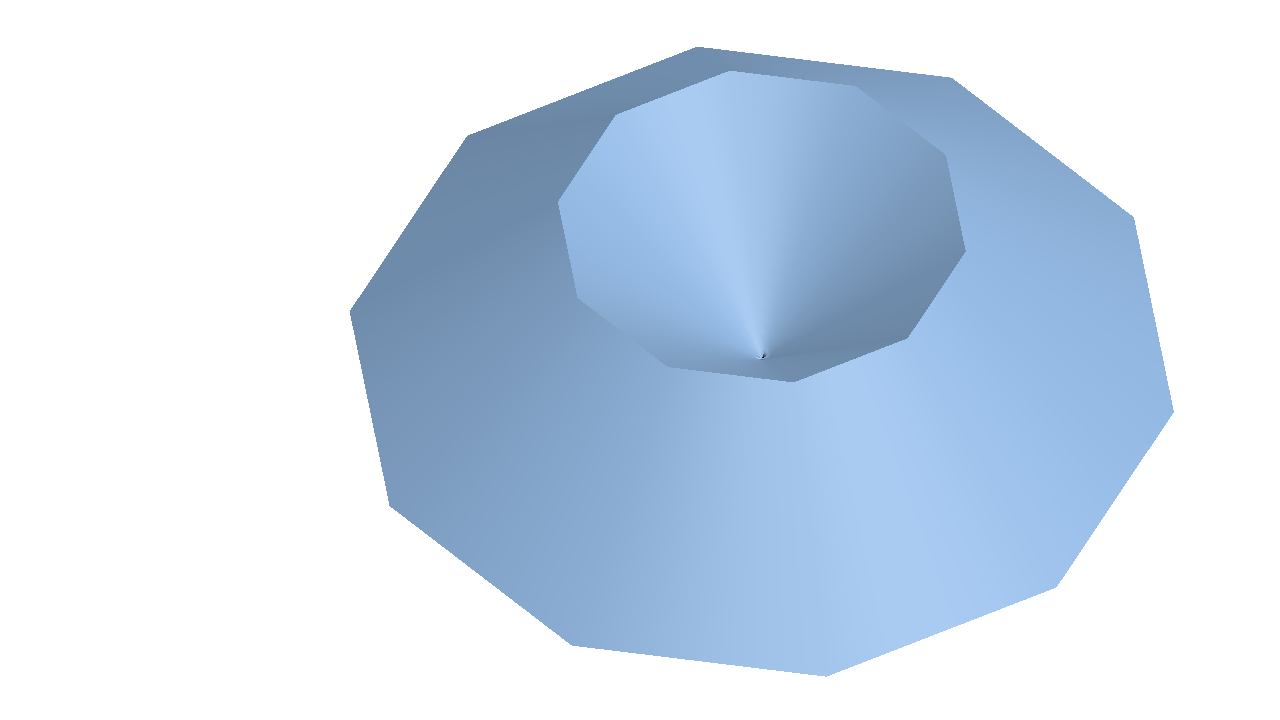
\includegraphics[width=70mm]{no/seg10.png}
    \end{center}
    \subcaption{セグメント数 : 10}
    \label{fig:s10}
  \end{minipage}
  \begin{minipage}{0.5\textwidth}
    \begin{center}
      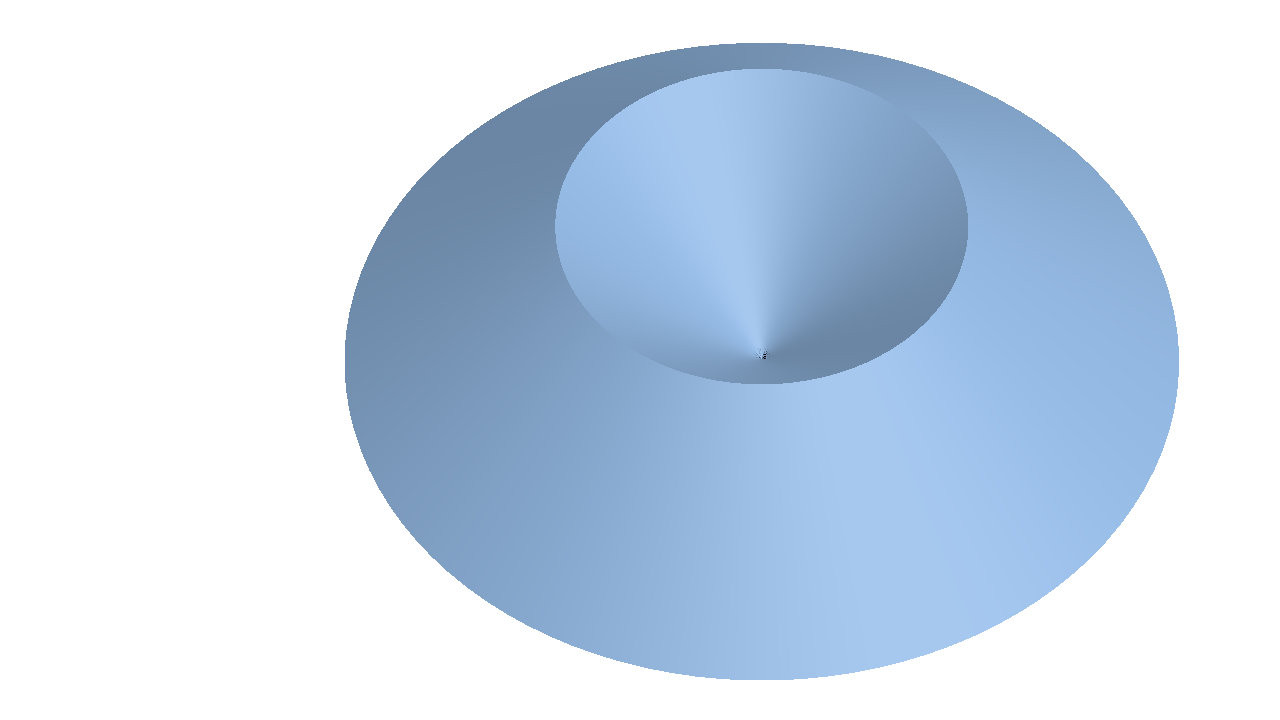
\includegraphics[width=70mm]{no/seg100.png}
    \end{center}
    \subcaption{セグメント数 : 100}
    \label{fig:s100}
  \end{minipage}
  \caption{正方形クリックのみ}
  \label{fig:seihou1no2}
\end{figure}
\begin{table}
  \caption{正方形の場合}
  \label{table:seiseg}
  \centering
  \begin{tabular}{|c|c|c|}
  \hline
  セグメント数 & ポリゴン数 & レンダリング時間\verb|(s)| \\
  \hline
  10 & 5296 & 0.52 \\
  20 & 6416 & 0.54 \\
  30 & 7536 & 0.53 \\
  40 & 8656 & 0.52 \\
  50 & 9776 & 0.54 \\
  60 & 10896 & 0.55 \\
  70 & 12016 & 0.53 \\
  80 & 13136 & 0.59 \\
  90 & 14256 & 0.58 \\
  100 & 15376 & 0.56 \\
  \hline
  \end{tabular}
\end{table}
三角形の場合も図\ref{fig:tri1no2}の画像左側を見れば分かりやすいが、角張り具合が減少している。また、表\ref{table:sanseg}からセグメント数が\ 45\ 増加するごとに、\ 1890\ 増加すると解かる。レンダリング時間も最大で0.01sの差であった。
\begin{figure}[htbp]
  \begin{minipage}{0.33\textwidth}
    \begin{center}
      \includegraphics[width=40mm]{no/notsquare-clock-segment10-420-009.png}
    \end{center}
    \subcaption{セグメント数 : 10}
    \label{fig:tris10}
  \end{minipage}
  \begin{minipage}{0.33\textwidth}
    \begin{center}
      \includegraphics[width=40mm]{no/notsquare-clock-segment55-2310-009.png}
    \end{center}
    \subcaption{セグメント数 : 55}
    \label{fig:tris55}
  \end{minipage}
  \begin{minipage}{0.33\textwidth}
    \begin{center}
      \includegraphics[width=40mm]{no/notsquare-clock-segment100-4200-010.png}
    \end{center}
    \subcaption{セグメント数 : 100}
    \label{fig:tris100}
  \end{minipage}
  \caption{三角形ドラッグのみ}
  \label{fig:tri1no2}
\end{figure}
\begin{table}
  \caption{三角形の場合}
  \label{table:sanseg}
  \centering
  \begin{tabular}{|c|c|c|}
  \hline
  セグメント数 & ポリゴン数 & レンダリング時間\verb|(s)| \\
  \hline
  10 & 420 & 0.09 \\
  55 & 2310 & 0.09 \\
  100 & 4200 & 0.10 \\
  \hline
  \end{tabular}
\end{table}

%
\subsection{考察}
%
概観の差分は図\ref{fig:seihou1no2}を見ると明らかであり、前者の外周が\ 10\ の角を持つことから、後者は恐らく\ 100\ の角を持つと推察される。つまり、スプライン曲線を回転させる際に、頂点を作成する回数を定義しているのがセグメント数と考えられる\verb|(|\ 360\ 度をセグメント数の値で割った角度ごとに作成\verb|)|\cite{3dsmaxspline}。そのため、セグメント数が変化すると、立体\verb|(スプライン曲線の回転体)|の周の滑らかさの観点で概観が異なって見えるのではないか。また、結果から、実験\ 1-2\ の考察のように、ポリゴン数の値をセグメント数との数式で表せると考え、ポリゴン数を\ P\ 、セグメント数を\ S\ とすると、正方形の場合は
\begin{equation}
  P = 1120S + 4176
\end{equation}
三角形の場合は、
\begin{equation}
  P = 42S
\end{equation}
と考察される。
%

\newpage
\section{実験\ 2}
長さ、幅、高さが\ 30\ で各セグメントが\ 1\ のボックスを作成し、次の作業の違いで、
概観の変化の仕方、ポリゴン数などにどういった差異が出るかを比較観察しなさい
\subsection{目的}
%
サブディビジョンの方法の違いによる、モデリング結果の差異を調査する
%
\subsection{方法や条件}
%
\begin{description}
\item{手順１} \verb|[作成]|パネルから、適当な大きさのボックスを作成
\item{手順２} \verb|[長さセグメント]|と\verb|[幅セグメント]|、\verb|[高さセグメント]|を\ 1\ に設定
\item{手順３} ボックスを選択し、\verb|[編集]|の\verb|[モデファイヤリスト]|から\verb|[メッシュスムーズ]|を選択
\item{手順４} \verb|[サブディビジョンの方法]|で\verb|[サブディビジョンの方法:]|を\verb|{従来型}|にし、\verb|[反復]|を\ 1\ ～\ 3\ にして、各々で実験\ 1\ -\ 1\ と同様にレンダリングを行う
\item{手順５} 手順４の\verb|[サブディビジョンの方法:]|を\verb|[四角形型]|や\verb|[NURMS]|にして行う
\item{手順６} レンダリング画像から概観を確かめる
\end{description}
%
\subsection{結果}
%
図\ref{fig:juuraigata}～図\ref{fig:nurmsgata}を観察すると、従来型は、サブディビジョンを行う前の立方体の頂点があった凡その位置を、それを三回行った後も認識できた。また、四角形型は立方体の各辺を半分に折り、各頂点の内角がすべて等しくなる様に調整しているように見える。更に、NURMS型は図\ref{fig:nurmsgata}から、この三つのサブディビジョンの中で、最も少ない反復で球体らしさが見られた。

\begin{figure}[htbp]
  \begin{minipage}{.33\textwidth}
    \begin{center}
      \includegraphics[width=35mm]{sub-juurai-1-004-24-26.png}
    \end{center}
    \subcaption{[反復 : 1}
    \label{fig:j1}
  \end{minipage}
  \begin{minipage}{.33\textwidth}
    \begin{center}
      \includegraphics[width=35mm]{sub-juurai-2-004-96-98.png}
    \end{center}
    \subcaption{反復 : 2}
    \label{fig:j2}
  \end{minipage}
  \begin{minipage}{.33\textwidth}
    \begin{center}
      \includegraphics[width=35mm]{sub-juurai-3-004-384-386.png}
    \end{center}
    \subcaption{反復 : 3}
    \label{fig:j3}
  \end{minipage}
  \caption{従来型}
  \label{fig:juuraigata}
\end{figure}
\begin{figure}[htbp]
  \begin{minipage}{.33\textwidth}
    \begin{center}
      \includegraphics[width=35mm]{sub-sikaku-1-004-26-24.png}
    \end{center}
    \subcaption{反復 : 1}
    \label{fig:si1}
  \end{minipage}
  \begin{minipage}{.33\textwidth}
    \begin{center}
      \includegraphics[width=35mm]{sub-sikaku-2-004-98-96.png}
    \end{center}
    \subcaption{反復 : 2}
    \label{fig:si2}
  \end{minipage}
  \begin{minipage}{.33\textwidth}
    \begin{center}
      \includegraphics[width=35mm]{sub-sikaku-3-004-386-384.png}
    \end{center}
    \subcaption{反復 : 3}
    \label{fig:si3}
  \end{minipage}
  \caption{四角形型}
  \label{fig:sikakkeigata}
\end{figure}
\begin{figure}[htbp]
  \begin{minipage}{.33\textwidth}
    \begin{center}
      \includegraphics[width=35mm]{sub-nurms-1-004-26-24.png}
    \end{center}
    \subcaption{[反復 : 1}
    \label{fig:n1}
  \end{minipage}
  \begin{minipage}{.33\textwidth}
    \begin{center}
      \includegraphics[width=35mm]{sub-nurms-2-004-98-96.png}
    \end{center}
    \subcaption{反復 : 2}
    \label{fig:n2}
  \end{minipage}
  \begin{minipage}{.33\textwidth}
    \begin{center}
      \includegraphics[width=35mm]{sub-nurms-3-004-386-384.png}
    \end{center}
    \subcaption{反復 : 3}
    \label{fig:n3}
  \end{minipage}
  \caption{NURMS型}
  \label{fig:nurmsgata}
\end{figure}

\newpage
表\ref{table:sikaku}と表\ref{table:nurms}より、四角形型と\ NURMS\ 型の頂点数及びポリゴン数は一致していると解かる。
更に、表\ref{table:juurai}～表\ref{table:nurms}から、四角形型と\ NURMS\ 型の頂点数とポリゴン数は、従来型の頂点数とポリゴン数を入れ替えた値になった。


\begin{table}
  \begin{minipage}{.30\textwidth}
  \caption{(従来型)反復数に伴う頂点数・ポリゴン数の変化}
  \label{table:juurai}
  \centering
  \begin{tabular}{|c|c|c|}
  \hline
  反復 & 頂点数 & ポリゴン数\\
  \hline
  1 & 24 & 26 \\
  2 & 96 & 98 \\
  3 & 384 & 386\\
  \hline
  \end{tabular}
  \end{minipage}
  \hfill
  \begin{minipage}{.30\textwidth}
  \caption{(四角形型)反復数に伴う頂点数・ポリゴン数の変化}
  \label{table:sikaku}
  \centering
  \begin{tabular}{|c|c|c|}
  \hline
  反復 & 頂点数 & ポリゴン数\\
  \hline
  1 & 26 & 24 \\
  2 & 98 & 96 \\
  3 & 386 & 384 \\
  \hline
  \end{tabular}
  \end{minipage}
  \hfill
  \begin{minipage}{.30\textwidth}
  \caption{(NURMS型)反復数に伴う頂点数・ポリゴン数の変化}
  \label{table:nurms}
  \centering
  \begin{tabular}{|c|c|c|}
  \hline
  反復 & 頂点数 & ポリゴン数\\
  \hline
  1 & 26 & 24 \\
  2 & 98 & 96 \\
  3 & 386 & 384 \\
  \hline
  \end{tabular}
  \end{minipage}
\end{table}
%
\newpage
\subsection{考察}
%
表\ref{table:sikaku}から、四角形型のポリゴン数は、反復の値が\ 1\ 増加するにつれ、\ 4\ 倍になっていることが解かる。ここから、四角形型が立方体の各辺を半分に折って新しく頂点を作成、それに伴い各面の中心も新しい頂点とし、この二種類の新しい頂点を繋ぐ辺を作成する方法だと仮説を立てる。簡潔にいうと、正方形の面を更に四つの正方形の面に分割する。これは、ポリゴン数が\ 4\ 倍になったことの整合性があう。さらに、それを裏付ける根拠は、表\ref{table:sikaku}の頂点数からも導ける。当たり前のことだが、四角形型のサブディビジョンを行う前の立方体の頂点数は\ 8\ であり、この仮説に基づいて、反復\ 1\ の四角形型の頂点数を計算すると、
\begin{gather*}
  \textrm{頂点数} + \textrm{面の中心(ポリゴン数)} + \textrm{頂点を結ぶ辺} + \textrm{面と辺を結ぶ辺} = \textrm{次の反復の頂点数} \\
  8 + 6 + 12 + 0 = 26 \textrm{(反復 1 の四角形型の頂点数)}
\end{gather*}
となり、表\ref{table:sikaku}のそれと一致するのである。さらに、反復\ 1\ から反復\ 2\ の四角形型の頂点数を計算すると、
\begin{equation*}
  26 + 24 + 24 + 24 = 98 \textrm{(反復 2 の四角形型の頂点数)}
\end{equation*}
となり、やはり一致する。よって、この仮説は正しいと考えられるのではないか。また、漸化式的に頂点数\ V\ を反復\ R\ とポリゴン数\ P\ 、辺の数\ S\ との関係式に起こしてみようと試みる\verb|(|$V_{R}$や$P_{R}$,$S_{R}$はその反復の値の時の頂点数とポリゴン数、辺数\verb|)|。下が成り立っていると推測する。
\begin{gather*}
  S_{0} = 12 \\
  P_{0} = 6 \\
  V_{0} = 8 \\
  S_{R} = 2S_{R-1} + 4P_{R-1} \\
  P_{R} = 4P_{R-1} \\
  V_{R} = V_{R-1} + P_{R-1} + S_{R-1}\\
  \text{ただし、$R\in{\mathbb{N}}$ とする}
\end{gather*}
  この漸化式は反復\ 1\ ～\ 3\ において正しいことを確認できた。
%

\newpage
\section{実験\ 3-1}
\verb|[ベースカラーと反射]|のところの色を様々に変化させ、どういった差異が出るかを観察しなさい
\subsection{目的}
%
\ 3\ dsMAX\ に備わっている色の編集機能を探求する
%
\subsection{方法や条件}
%
\begin{description}
  \item[手順１] \verb|[レンダリング]|のタブをクリックし、\verb|[マテリアルエディタ]|の\verb|[コンパクトマテリアルエディタ]|を開き、マテリアルを設定していないスロットを選択
  \item[手順２] \verb|[フィジカルマテリアル]|を使用し、\verb|[マテリアルモード:]|を\verb|[クラシック簡易]|にする
  \item[手順３] \verb|[コーティングパラメータ]|の\verb|[クリアコート]|の数字を\ 0.0\ に設定
  \item[手順４] \verb|[基本パラメータ]|の\verb|[ベースカラーと反射]|の位置にある、現在の色が表示されている正方形をクリックして、\verb|[赤:]|、\verb|[緑:]|、\verb|[青:]|をそれぞれ\ 1.0\ 、\ 0.8\ 、\ 0.1\ に設定
  \item[手順５] \verb|[ベースカラー]|、\verb|[光沢]|、\verb|[メタル:]|、\verb|[IOR;]|の数字をそれぞれ\ 0.8\ 、\ 0.3\ 、\ 0.0\ 、\ 1.0\ に設定
  \item[手順６] マテリアルを設定したスロットから、課題\ 4\ にて作成した\ CG\ にドラッグ＆ドロップでマテリアルを与える
  \item[手順７] \verb|[現実的マテリアルをビューポートに表示]|ボタンをオンにして、ビューポートにマップされた様子を表示
  \item[手順８] 手順\ 1\ ～\ 7\ までを再度行う。その際、手順\ 4\ の\verb|[赤:]|、\verb|[緑:]|、\verb|[青:]|をそれぞれ\ 0.3\ 、\ 0.7\ 、\ 0.0\ や\ 0.5\ 、\ 0.1\ 、\ 0.8\ に設定
  \item[手順９] レンダリング画像から概観を比較
\end{description}

%
\newpage
\subsection{結果}
%
課題\ 4\ で作成した\ CG\ に対して、図\ref{fig:iro3no1}では、手順に従ってマテリアルを与えた。また、図\ref{fig:g24311}と図\ref{fig:g24312}では、図\ref{fig:myellow}の明度と彩度を変更したマテリアルを与えた。

\begin{figure}[htbp]
  \begin{minipage}{.33\textwidth}
    \begin{center}
      \includegraphics[width=40mm]{material-100801-yel.png}
    \end{center}
    \subcaption{赤:1.0 緑:0.8 青:0.1}
    \label{fig:myellow}
  \end{minipage}
  \begin{minipage}{.33\textwidth}
    \begin{center}
      \includegraphics[width=40mm]{material-030700-grn.png}
    \end{center}
    \subcaption{赤:0.3 緑:0.7 青:0.0}
    \label{fig:mgreen}
  \end{minipage}
  \begin{minipage}{.33\textwidth}
    \begin{center}
      \includegraphics[width=40mm]{material-050108-pur.png}
    \end{center}
    \subcaption{赤:0.5 緑:0.1 青:0.8}
    \label{fig:mpurple}
  \end{minipage}
  \caption{RGBを変更}
  \label{fig:iro3no1}
\end{figure}
\begin{figure}[htbp]
  \begin{minipage}{.5\textwidth}
    \begin{center}
      \includegraphics[width=40mm]{yusou/2-4-3-1-1.png}
    \end{center}
    \subcaption{色設定画面}
    \label{fig:24311}
  \end{minipage}
  \begin{minipage}{.5\textwidth}
    \begin{center}
      \includegraphics[width=40mm]{2-4-3-1-1-v.png}
    \end{center}
    \subcaption{概観}
    \label{fig:24311v}
  \end{minipage}
  \caption{図\ref{fig:myellow}で彩度 0.9、明度 0.0}
  \label{fig:g24311}
\end{figure}
\begin{figure}[htbp]
  \begin{minipage}{.5\textwidth}
    \begin{center}
      \includegraphics[width=40mm]{yusou/2-4-3-1-2.png}
    \end{center}
    \subcaption{ 色設定画面}
    \label{fig:24312}
  \end{minipage}
  \begin{minipage}{.5\textwidth}
    \begin{center}
      \includegraphics[width=40mm]{2-4-3-1-2-v.png}
    \end{center}
    \subcaption{概観}
    \label{fig:24312v}
  \end{minipage}
  \caption{図\ref{fig:myellow}で彩度 0.0、明度 1.0}
  \label{fig:g24312}
\end{figure}
%
\subsection{考察}
%
図\ref{fig:24312}のように、彩度を\ 0.0\ に設定した場合、\ RGB\ が全て等しい数字に変化して、グレースケール上の色となったことから、\ RGB\ が互いの数字に差があることで、色彩豊かなカラーを再現できるのではないか。また、図\ref{fig:24311}のように、明度を\ 1.0\ に設定した場合、\ RGB\ 全ての数字が割合で値を増加させた。そのうち最も高い\ RGB\ の数字は\ 1.0\ となって、白色度合いを強めていたことから、\ RGB\ 全ての数字の合計が白色度合いの要素になるのではないか。
%

\newpage
\section{実験\ 3-2}
\verb|[ベースカラーと反射]|のところの数字を\ 0\ ～\ 1\ の間で様々に変化させ、どういった差異が出るかを観察しなさい
\subsection{目的}
%
\verb|[ベースカラーと反射]|の数字が、モデリングに与える色覚の影響を調査する
%
\subsection{方法や条件}
%
\begin{description}
  \item[手順１] 実験\ 3-1\ の手順\ 1\ ～\ 7\ までを行う
  \item[手順２] \verb|[ベースカラーと反射]|の数字を 0.0、 0.5、 1.0 と変化させ、その都度レンダリングを行う
  \item[手順３] 各々のレンダリング画像から概観を比較
\end{description}
%
\subsection{結果}
%
\verb|[ベースカラーと反射]|の数字が小さくなるにつれて、概観は黒色に変化した。
\begin{figure}[htbp]
  \begin{minipage}{.33\textwidth}
    \begin{center}
      \includegraphics[width=40mm]{basecolor-10.png}
    \end{center}
    \subcaption{ベースカラーと反射 : 1.0}
    \label{fig:bc10}
  \end{minipage}
  \begin{minipage}{.33\textwidth}
    \begin{center}
      \includegraphics[width=40mm]{basecolor-05.png}
    \end{center}
    \subcaption{ベースカラーと反射 : 0.5}
    \label{fig:bc05}
  \end{minipage}
  \begin{minipage}{.33\textwidth}
    \begin{center}
      \includegraphics[width=40mm]{basecolor-00.png}
    \end{center}
    \subcaption{ベースカラーと反射 : 0.0}
    \label{fig:bc00}
  \end{minipage}
  \caption{}
  \label{fig:bc3no2}
\end{figure}
%
\subsection{考察}
%
図\ref{fig:bc3no2}を比較検証すると、\verb|[ベースカラーと反射]|のパラメータが\ 1.0\ の場合がベースカラーの色であり、\ 0.0\ の場合は\ RGB\ 全て\ 0\ の図\ref{fig:24311v}と概観が全く同じになったことから、このパラメータは、その右横にある色表示パネルの RGB 成分を\ 1\verb|(百分率)|\ としたときに、その数字を百分率の割合として、光を反射すると考えられる。富永昌治(1992)によると、物体表面や内部色素による光の反射の仕方が物体に質感を持たせているという\cite{tominaga}。このパラメータは作成したい\ CG\ の材質を再現する重要な要素だと考えられる。
%

\newpage
\section{実験\ 3-3}
\verb|[粗さ](光沢)|を\ 0\ ～\ 1\ の間で、\ IOR\ を\ 1\ ～\ 10\ の間で様々に変化させ、どういった差異が出るかを観察しなさい
\subsection{目的}
%
粗さと\ IOR\ が、モデリングに与える色覚の影響を調査する
%
\subsection{方法や条件}
%
\begin{description}
  \item[手順１] 実験\ 3-1\ の手順\ 1\ ～\ 7\ までを行う
  \item[手順２] \verb|[粗さ](初期設定)|を\verb|[光沢]|に変更
  \item[手順３] \verb|[光沢]|の数字は\ 0.5\ 、\verb|[IOR]|の数字は\ 1.0\ 、\ 5.0\ 、\ 10.0\ から設定し、全ての組み合わせでレンダリングを行う
  \item[手順４] \verb|[IOR]|の数字は\ 5.0\ 、\verb|[光沢]|の数字は\ 0.1\ 、\ 0.5\ 、\ 1.0\ から設定し、全ての組み合わせでレンダリングを行う
  \item[手順５] 各々のレンダリング画像から概観を比較
\end{description}
%
\subsection{結果}
%
図\ref{fig:koutaku05}～図\ref{fig:ior05} を観察すると、\verb|[光沢]|の数字を増加させるにつれ、画像全体の反射光の白っぽさが減少していることと、逆に、\verb|[IOR]|の数字を増加させるとオブジェクトの端の部分の白っぽさが増加していることが解かる。
\begin{figure}[htbp]
  \begin{minipage}{.33\textwidth}
    \begin{center}
      \includegraphics[width=40mm]{koutakuiorr-05-01.png}
    \end{center}
    \subcaption{IOR : 1.0}
    \label{fig:c05i01}
  \end{minipage}
  \begin{minipage}{.33\textwidth}
    \begin{center}
      \includegraphics[width=40mm]{koutakuiorr-05-05.png}
    \end{center}
    \subcaption{IOR : 5.0}
    \label{fig:c05i05no1}
  \end{minipage}
  \begin{minipage}{.33\textwidth}
    \begin{center}
      \includegraphics[width=40mm]{koutakuiorr-05-10.png}
    \end{center}
    \subcaption{IOR : 10.0}
    \label{fig:c05i10}
  \end{minipage}
  \caption{光沢を 0.5 に固定}
  \label{fig:koutaku05}
\end{figure}
\begin{figure}[htbp]
  \begin{minipage}{.33\textwidth}
    \begin{center}
      \includegraphics[width=40mm]{koutakuiorr-01-05.png}
    \end{center}
    \subcaption{光沢 : 0.1}
    \label{fig:c01i05}
  \end{minipage}
  \begin{minipage}{.33\textwidth}
    \begin{center}
      \includegraphics[width=40mm]{koutakuiorr-05-05.png}
    \end{center}
    \subcaption{光沢 : 0.5}
    \label{fig:c05i05no2}
  \end{minipage}
  \begin{minipage}{.33\textwidth}
    \begin{center}
      \includegraphics[width=40mm]{koutakuiorr-10-05.png}
    \end{center}
    \subcaption{光沢 : 1.0}
    \label{fig:c10i05}
  \end{minipage}
  \caption{ IOR を 5.0 に固定}
  \label{fig:ior05}
\end{figure}
%
\subsection{考察}
%
Autodesk(2023)によると、\verb|[粗さ]|の数字を高くした場合は、ぼやけたマテリアルになり、低くした場合は、鏡のようなマテリアルになるといい、さらに、\verb|[粗さ]|と\verb|[光沢]|の関係は反転しているという\cite{3dsmaxkoutaku}。つまり、図\ref{fig:c01i05}の白っぽさが他の画像に比べて強いことの理由が、\verb|[光沢]|の値が低く、ぼやけているように見えたと考えられる。
%

\newpage
\section{実験\ 4-1}
\verb|[基本パラメータ]|のところで、\verb|[ベースカラーと反射]|のみを設定する、\verb|[透明度]|のみを設定する、\verb|[ベースカラーと反射]|と\verb|[透明度]|を両方を設定する
\subsection{目的}
%
\verb|[ベースカラーと反射]|や\verb|[透明度]|を変更したマテリアルが、オブジェクトの概観をどのように変化させるか調査する
%
\subsection{方法や条件}
%
\begin{description}
  \item[手順１] \verb|[標準プリミティブ]|の\verb|[平面]|を選択
  \item[手順２] 適当な方眼の格子点を原点としたときの相対座標\verb|{-4, 0}|から\verb|{0, 4}|へドラッグし生成
  \item[手順３] \verb|[球]|を選択し、半径\ 1.8\ と入力し生成
  \item[手順４] 手順\ 2\ で生成した\verb|[平面]|をもう三つ複製、\verb|[平面]|を図\ref{fig:341n}のように平行に並べる
  \item[手順５] 球オブジェクトを選択
  \item[手順６] \verb|[レンダリング]|から\verb|[マテリアルエディタ]|、\verb|[コンパクトマテリアルエディタ]|を開き、マテリアルを設定していないスロットを選択
  \item[手順７] \verb|[基本パラメータ]|から\verb|[ベースカラー]|、\verb|[粗さ]|、\verb|[メタル]|、\verb|[透明度]|の数字をそれぞれ、\ 0.8\ 、\ 0.0\ 、\ 0.0\ 、\ 0.8\ に設定
  \item[手順８] \verb|[薄壁]|にチェックを入れる
  \item[手順９] このマテリアルを作成した球オブジェクトに適用。また、手順\ 7\ と同じマテリアルを別途作成し平面に与える。しかし、これ以降の手順では球のマテリアルを設定する
  \item[手順１０] \verb|[ベースカラーと反射]|の色表示右側にある正方形をクリックし\verb|[ビットマップ]|を選択しグラデーション画像のファイルを与える。この際、用いるグラデーション画像はバナー工房\url{https://www.bannerkoubou.com/photoeditor/gradation/}で作成する。そして一度レンダリングを行う
  \item[手順１１] \verb|[親に戻る]|ボタンを押し、\verb|[基本パラメータ]|のところで\verb|[ベースカラーと反射]|を\ 0.0\ 、\ 0.5\ 、\ 1.0\ に設定し、各々レンダリングを行う
  \item[手順１２] \verb|[ベースカラーと反射]|を\ 0.8\ に戻し、今度は\verb|[透明度]|を\ 0.0\ 、\ 0.5\ 、\ 1.0\ に設定し、各々ビューポートから確かめる
  \item[手順１３] \verb|[透明度]|を\ 0.8\ に戻し、\verb|[ベースカラーと反射]|と\verb|[ベースカラーと反射]|を\ 0.0\ 、\ 0.5\ 、\ 1.0\ に設定し、各々レンダリングを行う
  \item[手順１４] 各々のレンダリング画像から概観を比較
\end{description}

\begin{figure}[htbp]
  \begin{center}
    \includegraphics[width=70mm]{3-4-1-normal.png}
  \end{center}
  \caption{平面と球の配置}
  \label{fig:341n}
\end{figure}
%
\newpage
\subsection{結果}
%
図\ref{fig:bc08t08}は手順\ 1\ ～\ 10\ の実行結果であり、
\begin{figure}[htbp]
    \begin{center}
      \includegraphics[width=70mm]{0808.png}
    \end{center}
    \caption{ベースカラーと反射 : 0.8, 透明度 : 0.8}
    \label{fig:bc08t08}
\end{figure}
図\ref{fig:toumei08}は手順\ 11\ の実行結果である。
\begin{figure}[htbp]
  \begin{minipage}{.33\textwidth}
    \begin{center}
      \includegraphics[width=40mm]{0008.png}
    \end{center}
    \subcaption{ベースカラーと反射 : 0.0}
    \label{fig:bc00t08}
  \end{minipage}
  \begin{minipage}{.33\textwidth}
    \begin{center}
      \includegraphics[width=40mm]{0508.png}
    \end{center}
    \subcaption{ベースカラーと反射 : 0.5}
    \label{fig:bc05t08}
  \end{minipage}
  \begin{minipage}{.33\textwidth}
    \begin{center}
      \includegraphics[width=40mm]{1008.png}
    \end{center}
    \subcaption{ベースカラーと反射 : 1.0}
    \label{fig:bc10t08}
  \end{minipage}
  \caption{透明度を 0.8 に固定}
  \label{fig:toumei08}
\end{figure}

図\ref{fig:basecolor08}は手順\ 12\ の実行結果である。
\begin{figure}[htbp]
  \begin{minipage}{.33\textwidth}
    \begin{center}
      \includegraphics[width=40mm]{0800.png}
    \end{center}
    \subcaption{透明度 : 0.0}
    \label{fig:bc08t00}
  \end{minipage}
  \begin{minipage}{.33\textwidth}
    \begin{center}
      \includegraphics[width=40mm]{0805.png}
    \end{center}
    \subcaption{透明度 : 0.5}
    \label{fig:bc08t05}
  \end{minipage}
  \begin{minipage}{.33\textwidth}
    \begin{center}
      \includegraphics[width=40mm]{0810.png}
    \end{center}
    \subcaption{透明度 : 1.0}
    \label{fig:bc08t10}
  \end{minipage}
  \caption{ベースカラーと反射を 0.8 に固定}
  \label{fig:basecolor08}
\end{figure}

図\ref{fig:3no3ryouhou}は手順\ 13\ の実行結果である。
\begin{figure}[htbp]
  \begin{minipage}{.33\textwidth}
    \begin{center}
      \includegraphics[width=40mm]{0000_.png}
    \end{center}
    \subcaption{ベースカラーと反射 : 0.0, 透明度 : 0.0}
    \label{fig:bc00t00}
  \end{minipage}
  \begin{minipage}{.33\textwidth}
    \begin{center}
      \includegraphics[width=40mm]{0505.png}
    \end{center}
    \subcaption{ベースカラーと反射 : 0.5, 透明度 : 0.5}
    \label{fig:bc05t05}
  \end{minipage}
  \begin{minipage}{.33\textwidth}
    \begin{center}
      \includegraphics[width=40mm]{1010.png}
    \end{center}
    \subcaption{ベースカラーと反射 : 1.0, 透明度 : 1.0}
    \label{fig:bc10t10}
  \end{minipage}
  \caption{両方を設定}
  \label{fig:3no3ryouhou}
\end{figure}
%
\newpage
\subsection{考察}
%
図\ref{fig:bc00t08}図\ref{fig:bc08t10}、図\ref{fig:bc10t10}は、平面上部からの球の影が見られない。そのため、\verb|[ベースカラーと反射]|の値を\ 0.0\ にした場合や\verb|[透明度]|の値を\ 1.0\ にした場合に、球からの反射光が存在しないと考えられる。これは、平面が重なっていない球の部分が黒色であることからも解かるだろう。また、\verb|[ベースカラーと反射]|はオブジェクトの表面で反射した光の強さ、\verb|[透明度]|は降り注ぐ光のオブジェクトを透過する割合とし、オブジェクトを透過しなかった光のみ反射が可能と仮説を立てる。もし仮説が正しいとしたら、\verb|[ベースカラーと反射]|を\ B\ 、\verb|[透明度]|を\ I\ 、オブジェクトの反射光の強さを\ S\ とすると\verb|(降り注ぐ光の強さを 1 とし)|、
\begin{equation*}
  S = B(1 - I)
\end{equation*}
で表せる関係ではないかと考えられる。そのため、図\ref{fig:bc08t08}と図\ref{fig:toumei08}、図\ref{fig:3no3ryouhou}の全ての画像を計算することで調査する。表\ref{table:keisan}は、反射光の強さの順位を見た目上と計算上の両方を記載した計算結果である。表\ref{table:keisan}の一行目と三行目は人間の目には反射光の強さが同じに見えたが、計算上では\ 0.06\ 違っている。しかし、その点を除いて一致しているため、この式は目安としては十分正確だと考えられるのではないか。
\begin{table}
  \caption{計算結果}
  \label{table:keisan}
  \centering
  \begin{tabular}{|c|c|c|c|}
  \hline
  図 & 光の強さ(S) & 見た目上の順位(反射光) & 計算上の順位(反射光)\\
  \hline
  \ref{fig:bc08t08} & 0.16 & 5 & 5 \\
  \ref{fig:bc00t08} & 0.00 & 7 & 7 \\
  \ref{fig:bc05t08} & 0.10 & 5 & 6 \\
  \ref{fig:bc10t08} & 0.20 & 4 & 4 \\
  \ref{fig:bc08t00} & 0.80 & 1 & 1 \\
  \ref{fig:bc08t05} & 0.40 & 2 & 2 \\
  \ref{fig:bc08t10} & 0.00 & 7 & 7 \\
  \ref{fig:bc00t00} & 0.00 & 7 & 7 \\
  \ref{fig:bc05t05} & 0.25 & 3 & 3 \\
  \ref{fig:bc10t10} & 0.00 & 7 & 7 \\
  \hline
  \end{tabular}
\end{table}
%

\newpage
\section{実験\ 4-2}
\verb|[レンダリング]|のメニューから\verb|[レンダリング設定]|のウィンドウを出して、\verb|[Arnold Renderer]|のタブで、\verb|[Depth Limit]|の\verb|[Ray Limit Total:]|を\ 0\ ～\ 5\ に\ 1\ ずつ変化させる\verb|(レイトレースの光がどこまでの深さを計算するかという透過の回数でできる画像がどう変わるか)|
\subsection{目的}
%
レイトレースの光の計算する深さの数字のみを変更したとき、概観にどのような影響が見られるか調査する
%
\subsection{方法や条件}
%
各種条件は実験\ 4-1\ の手順にて記載されている
\begin{description}
  \item[手順１] 実験\ 4-1\ の手順\ 1\ ～\ 10\ までを行う
  \item[手順２] \verb|[レンダリング]|のメニューから\verb|[レンダリング設定]|のウィンドウを開く
  \item[手順３] \verb|[Arnold Renderer]|のタブで、\verb|[Depth Limit]|の\verb|[Ray Limit Total:]|を\ 0\ ～\ 5\ に\ 1\ ずつ変化させ、各々でレンダリングを行う
  \item[手順４] 各々のレンダリング画像から概観を比較する 
\end{description}
%
\subsection{結果}
%
図\ref{fig:dep0kara2}～図\ref{fig:dep3kara5}を観察すると、図\ref{fig:d0}～図\ref{fig:d2}までは、レイトレースの光が透過可能なオブジェクトの個数は、その\ Depth\ の値と一致すると解かる。しかし、図\ref{fig:d3}～図\ref{fig:d5}は同じ概観になった。
\begin{figure}[htbp]
  \begin{minipage}{.33\textwidth}
    \begin{center}
      \includegraphics[width=40mm]{s3-4-2-0.png}
    \end{center}
    \subcaption{Depth : 0}
    \label{fig:d0}
  \end{minipage}
  \begin{minipage}{.33\textwidth}
    \begin{center}
      \includegraphics[width=40mm]{s3-4-2-1.png}
    \end{center}
    \subcaption{Depth : 1}
    \label{fig:d1}
  \end{minipage}
  \begin{minipage}{.33\textwidth}
    \begin{center}
      \includegraphics[width=40mm]{s3-4-2-2.png}
    \end{center}
    \subcaption{Depth : 2}
    \label{fig:d2}
  \end{minipage}
  \caption{概観の変化がみられる}
  \label{fig:dep0kara2}
\end{figure}
\begin{figure}[htbp]
  \begin{minipage}{.33\textwidth}
    \begin{center}
      \includegraphics[width=40mm]{s3-4-2-3.png}
    \end{center}
    \subcaption{Depth : 3}
    \label{fig:d3}
  \end{minipage}
  \begin{minipage}{.33\textwidth}
    \begin{center}
      \includegraphics[width=40mm]{s3-4-2-4.png}
    \end{center}
    \subcaption{Depth : 4}
    \label{fig:d4}
  \end{minipage}
  \begin{minipage}{.33\textwidth}
    \begin{center}
      \includegraphics[width=40mm]{s3-4-2-5.png}
    \end{center}
    \subcaption{Depth : 5}
    \label{fig:d5}
  \end{minipage}
  \caption{概観の変化がみられない}
  \label{fig:dep3kara5}
\end{figure}
%
\newpage
\subsection{考察}
%
図\ref{fig:dep3kara5}の概観が変化しなかった理由を考察する。この実験における平面は各々互いに平行に設置されていたが、レンダリングの視点位置が、\ 3\ つ以上のオブジェクト透過する光を得られない不適切な位置であったためだと考えられる。つまり、平面に対して垂直に近い必要があったのである。また、仕組み上\verb|[Depth]|の数字を大きくするに連れて、演算回数が増加することはほぼ自明である。そのため、\verb|[Depth]|の数字を目的に対して十分かつ、大きすぎないように設定することが、レンダリング時間削減等に繋がるのではないか。
%

\newpage
\section{実験\ 4-3}
\verb|[Arnold Renderer]|のタブで、\verb|[Adaptive and Progressive]|のところで、\verb|[Adaptive Sampling]|にチェックを入れたりチェックを外したりして切り替える\verb|(これでエイリアシングの発生、アンチエイリアシング処理の効果を見る)|
\subsection{目的}
%
\ 3dsMax\ のエイリアシング発生及びアンチエイリアシング処理の効果を調査する
%
\subsection{方法や条件}
%
各種条件は実験\ 4-1\ の手順にて記載されている
\begin{description}
  \item[手順１] 実験\ 4-1\ の手順\ 1\ ～\ 10\ までを行う
  \item[手順２] \verb|[レンダリング]|のメニューから\verb|[レンダリング設定]|のウィンドウを開く
  \item[手順３] \verb|[Arnold Renderer]|のタブで、\verb|[Adaptive and Progressive]|のところで\verb|[Adaptive Sampling]|にチェックを入れ、レンダリングを行う
  \item[手順４] \verb|[Adaptive Sampling]|のチェックを外し、レンダリングを行う
  \item[手順５] レンダリング画像から概観を確認する
\end{description}
%
\subsection{結果}
%
図\ref{fig:ason}は\verb|[Adaptive Sampling]|のチェックを入れており、図\ref{fig:asoff}はそれを入れていない同一の\ 3D\ オブジェクトのレンダリング画像である。
また、図\ref{fig:fason}と図\ref{fig:fasoff}はそれぞれの端の拡大画像であり、両方とも、理由は解らないがアンチエイリアシング処理されていた。しかし、レンダリング時間は異なり、順に\ 24\ s、\ 16\ sであった。
\begin{figure}[htbp]
  \begin{minipage}{.50\textwidth}
    \begin{center}
      \includegraphics[width=70mm]{s3-4-3-on.png}
    \end{center}
    \subcaption{on}
    \label{fig:ason}
  \end{minipage}
  \begin{minipage}{.50\textwidth}
    \begin{center}
      \includegraphics[width=70mm]{s3-4-3-off.png}
    \end{center}
    \subcaption{off}
    \label{fig:asoff}
  \end{minipage}
  \caption{Adaptive Sampling}
  \label{fig:adaptive}
\end{figure}

\begin{figure}[htbp]
  \begin{minipage}{.50\textwidth}
    \begin{center}
      \includegraphics[width=70mm]{antiareas-on.png}
    \end{center}
    \subcaption{on}
    \label{fig:fason}
  \end{minipage}
  \begin{minipage}{.50\textwidth}
    \begin{center}
      \includegraphics[width=70mm]{antiareas-off.png}
    \end{center}
    \subcaption{off}
    \label{fig:fasoff}
  \end{minipage}
  \caption{端を拡大した図\ref{fig:adaptive}}
  \label{fig:fadaptive}
\end{figure}
%
\newpage
\subsection{考察}
%
様々なモデルで何度も試した結果、\verb|[Adaptive and Sampling]|のチェックを入れていない場合でも、出力画像のアンチエイリアシング処理が行われていることを確認した。このため、\verb|[Adaptive and Sampling]|はアンチエイリアシング処理を行っているわけではないのではないか。また、アンチエイリアシング処理の効果の考察は可能であるため行うこととする。
図\ref{fig:adaptive}は、画素の色が変化する部分の境目が滑らかである。そのため、違和感が感じられにくい。その仕組みは、図\ref{fig:fadaptive}から、二つの異なる色の境目に色の緩衝のため中間色を入れ、色調変化を滑らかにしている。こうして、極端な色調変化による違和感を抑制していると考えられる。
%

\newpage
\begin{thebibliography}{9}
  \bibitem{toritchi}
    とりっち. "描画したスプラインのカーブが滑らかでない (3ds Max の使い方 操作方法 Tips)". iPentec. 2022. \\
    \url{https://www.ipentec.com/document/3ds-max-spline-curve-is-not-smooth}, (参照 2023-11-06).
  \bibitem{Aismiley}
    Aismiley編集部. "AI・人工知能ができること、できないこと。人間にしかできない仕事は？". Aismiley. 2023. \\
    \url{https://aismiley.co.jp/ai_news/what-ai-can-not-do/}, (参照 2023-11-06).
  \bibitem{moriya}
    守屋悦朗. "与えられた点によって定まる滑らかな曲線の描き方". 早稲田大学. (2023)\\ 
\url{https://www.f.waseda.jp/moriya/PUBLIC_HTML/education/classes/infomath6/applet/fractal/spline/}, (参照 2023-11-18).
  \bibitem{cgworld}
    CGWORLD.jp. "テクスチャマップの理解". CGWORLD.jp. 2016
\url{https://cgworld.jp/feature/1602-3dtotal-digitaltutors-2.html}, (参照 2023-11-19)
  \bibitem{3dsmaxspline}
    Autodesk. "3ds Max 2024 ヘルプ | Spring". Autodesk. 2023
\url{https://help.autodesk.com/view/3DSMAX/2024/JPN/?guid=GUID-11C7253F-EF59-4312-9991-7C13B5968112}, (参照 2023-11-19)
  \bibitem{3dsmaxkoutaku}
    Autodesk. "[基本パラメータ](Basic Parameters)ロールアウト(フィジカル マテリアル)". Autodesk. 2023
\url{https://help.autodesk.com/view/3DSMAX/2024/JPN/?guid=GUID-B8A945E2-3C37-4A7A-90FA-D7209BE59643}, (参照 2023-11-20)
  \bibitem{tominaga}
    富永昌治, and 大橋伸一郎. "物体のカラー反射モデル". 情報処理学会論文誌 33.1 (1992): 37-45. (参照 2023-11-17)
  \bibitem{tanaka}
    田中敏光, and 高橋時市郎. "アンチ・エリアシングのための直交スキャンライン法". 情報処理学会論文誌 32.2 (1991): 197-205. (参照 2023-11-20)
  \bibitem{nvidia}
    Nvidia. "アンチエイリアシング". Nvidia. (掲載年不明)
\url{https://www.nvidia.com/content/control-panel-help/vlatest/ja-jp/mergedprojects/nv3djpn/antialiasing.htm}, (参照 2023-11-20)
\end{thebibliography}

\end{document}
